%%%%%%%%%%%%%%%%%%%%%%%%%%%%%%%%%%%%%%%%%%%%%%%%%%%%%%%%%%%%%%%%%%%%%%
% LaTeX Template: Curriculum Vitae
%
% Source: http://www.howtotex.com/
% Feel free to distribute this template, but please keep the
% referal to HowToTeX.com.
% Date: July 2011
% 
%%%%%%%%%%%%%%%%%%%%%%%%%%%%%%%%%%%%%%%%%%%%%%%%%%%%%%%%%%%%%%%%%%%%%%
% How to use writeLaTeX: 
%
% You edit the source code here on the left, and the preview on the
% right shows you the result within a few seconds.
%
% Bookmark this page and share the URL with your co-authors. They can
% edit at the same time!
%
% You can upload figures, bibliographies, custom classes and
% styles using the files menu.
%
% If you're new to LaTeX, the wikibook is a great place to start:
% http://en.wikibooks.org/wiki/LaTeX
%
%%%%%%%%%%%%%%%%%%%%%%%%%%%%%%%%%%%%%%%%%%%%%%%%%%%%%%%%%%%%%%%%%%%%%%

%%%%%%%%%%%%%%%%%%%%%%%%%%%%%%%%%%%%%%%%%%%%%%%%%%%%%%%%%%%%%%%%%%%%%%
% Specify the type of the document
% document type alternative: article,report,book and slides
%%%%%%%%%%%%%%%%%%%%%%%%%%%%%%%%%%%%%%%%%%%%%%%%%%%%%%%%%%%%%%%%%%%%%%
\documentclass[paper=a4,fontsize=11pt]{scrartcl} % KOMA-article class

%%% Call macro sets				
\usepackage[english]{babel}

%%% Character Encode
\usepackage[utf8]{inputenc}                   % 替换你正在使用的编码
\usepackage{CJKutf8}

\usepackage[protrusion=true,expansion=true]{microtype}
\usepackage{amsmath,amsfonts,amsthm}     % Math packages
\usepackage{graphicx}                    % Enable pdflatex
\usepackage[svgnames]{xcolor}            % Colors by their 'svgnames'
\usepackage{geometry}
	\textheight=700px                   % Saving trees ;-)
\usepackage{url}
\usepackage{multicol}                    % multiple columns

\frenchspacing                           % Better looking spacings after periods
\pagestyle{empty}                        % No pagenumbers/headers/footers

%%% Custom sectioning (sectsty package)
%%% ------------------------------------------------------------
\usepackage{sectsty}

\sectionfont{%			              % Change font of \section command
	\usefont{OT1}{phv}{b}{n}%		   % bch-b-n: CharterBT-Bold font
	\sectionrule{0pt}{0pt}{-10pt}{3pt}}

%%% Macros
%%% ------------------------------------------------------------
\newlength{\spacebox}
\settowidth{\spacebox}{8888888888}			% Box to align text
\newcommand{\sepspace}{\vspace*{1em}}		% Vertical space macro

\newcommand{\Title}[1]{ % Name
		\begin{center}
			\Huge #1
		\end{center}
		\par \normalsize \normalfont} % \par 换行
		
\newcommand{\Slogan}[1]{ % Slogan (optional)
		\large \usefont{OT1}{phv}{m}{n}\hfill \textit{#1} % \textit italic text
		\par \normalsize \normalfont}

\newcommand{\Section}[1]{\section*{ #1 }}          % * 去掉section标号

\newcommand{\SubSection}[2]{
	\sepspace \noindent \textbf{#1} \hfill      % 项目名称
	\colorbox{Black}{\parbox{7em}{\hfill\color{White}#2}} \par  % 时间
	\normalsize \par \sepspace}


\newcommand{\Personal}[2]{
		\noindent\hangindent=2em\hangafter=0 % Indentation
		\parbox{\spacebox}{#1}     % Box to align text		       
		\hspace{1.5em} #2 \par}    % Entry value

\newcommand{\Education}[3]{
		\noindent \textbf{#1} \hfill      % \textbf 加粗
		\colorbox{Black}{%
		\parbox{7em}{%
		\hfill\color{White}#2}} \par  % Duration
		#3
		\normalsize \par}

\newcommand{\Work}[3]{
		\noindent \textbf{#1} \hfill      % 公司名称
		\colorbox{Black}{\parbox{7em}{\hfill\color{White}#2}} \par  % 时间
		#3 \par              % 职位
		\normalsize \par}

\newcommand{\Academic}[2]{
		\noindent \textbf{#1} \par      % 分类
		\hangindent=2em \small #2 % 成果项
		\normalsize \par}

%%% Begin Document
%%% ------------------------------------------------------------
\begin{document}
\begin{CJK}{UTF8}{gbsn}                       % 详情参阅CJK文件包
% you can upload a photo and include it here...
%\begin{wrapfigure}{l}{0.5\textwidth}
%	\vspace*{-2em}
%		\includegraphics[width=0.15\textwidth]{photo}
%\end{wrapfigure}

\Title{个人简历}
% \MySlogan{RubyChina}

\sepspace % set spacing between lines

%%% Personal details
%%% ------------------------------------------------------------
\Section{基本信息}

\begin{multicols}{2}                           % 分两栏
\Personal{姓 名}{姜政冬}
\Personal{电 话}{18668150635}
\Personal{邮  箱}{\url{xautjzd@gmail.com}}
\Personal{住  址}{浙江省杭州市}
\Personal{GitHub}{https://github.com/xautjzd}
\Personal{英 语}{CET-6}

\columnbreak                                   % 强制分栏
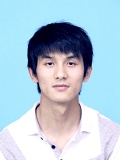
\includegraphics[width=0.2\textwidth\hfill]{xautjzd1.jpg}
\end{multicols}

%%% Education
%%% ------------------------------------------------------------
\Section{教育经历}

\Education{西安理工大学}{2012.09-2015.07}{专业: 软件工程 学历: 硕士(保送)}
\sepspace
\Education{西安理工大学}{2008.08-2012.06}{专业: 网络工程 学历: 学士}

%%% Work
%%% ------------------------------------------------------------
\Section{工作经历}

\Work{阿里云端点科技-低代码平台}{2020.07-现在}{资深 Java 开发工程师}
\Work{阿里云端点科技-Paas 平台}{2018.07-2020.06}{资深 Golang 开发工程师}
\sepspace
\Work{杭州网易网络有限公司-网易云容器服务}{2015.07-2018.07}{高级 Java 开发工程师}

%%% Project
%%% ------------------------------------------------------------
\Section{项目经历}

\SubSection{低代码平台}{2020.07-现在}
项目描述: Trantor 是一个中后台业务应用的快速研发与交付体系,通过对应用、交互 \& 场景的抽象,以元数据驱动的方式为业务应用开发提效,主要抽象了模型、逻辑、视图三大类资源,其中模型主要用于承载业务数据,逻辑为业务流程编排的抽象,可方便二开,视图抽象了一套 DSL,以便后端开发快速实现数据的展示。\par
\sepspace
项目职责:
\begin{itemize}
\item 负责 Trantor 核心机制开发,包括场景抽象、元数据采集、业务流程编排、模型触发器、i18n 等机制开发。
\item 负责后端研发规范制定 \& 落地。
\end{itemize}

\SubSection{端点 PaaS 平台}{2018.07-2020.06}
项目描述:端点 PaaS 平台(名为 Erda)基于 Docker \& Kubernetes 构建(之前采用 DC/OS Marathon \& Mesos),提供了源码托管、CI/CD、中间件管理、微服务治理、快数据、运维监控、测试平台等功能,有效地提高企业的 IT 研发、运维、运营效率,降低成本。遵循基础设施及代码理念,抽象了 pipeline.yml \& dice.yml,分别用于描述 CI 场景 \& CD 场景,其中 CI 抽象与 GitHub Workflow/Travis CI 类似,节点功能可自行扩展,CD 抽象包含服务所需 cpu \& memory、副本数、暴露端口、依赖中间件等,一键拉起所有服务, 支持 SaaS 化部署与私有化部署两种方式。\par
\sepspace
项目职责:  
\begin{itemize}
\item 负责抽象并维护 Erda 部署所需制品。
\item 负责开发并维护 Erda cli(基于 cobra),将 CI/CD、市场推送等关键能力通过 cli 提供给用户,为用户提效。
\item 负责开发并维护 pipeline.yml 常用场景所需的 actions,如(java 构建、javascript 构建、git-checkout 等)。
\item 负责开发并维护 Erda 平台的各种元信息(如企业、项目、应用、Runtime、Service、实例等)。
\item 负责 Erda 调度器插件 Spark/Flink 的开发,支持通过 Erda 将任务提交至 Spark/Flink 平台。
\item 作为核心主力完成 Erda 平台从早期 Kotlin 到 Go 重构,及底层编排引擎从 DC/OS(Mesos) 到 Kubernetes 的迁移。 
\end{itemize}

\SubSection{网易云容器平台}{2015.07-2018.07}
项目描述: 网易云容器平台作为网易云的子产品,基于网易内部 Iaas 平台 \& Kubernetes 提供公有云容器服务 \& 公有云镜像仓库,具体包括有状态工作负载、无状态工作负载、服务发现、云盘挂载、弹性公网 IP 绑定、镜像构建、上传、下载、分享等功能。另外,团队还承担整个网易云控制台开发,包括各垂直服务接入、API 流控、服务灰度发布等。\par
\sepspace
项目职责:
\begin{itemize}
\item 负责 Namespace 生命周期管理、Deployment 生命周期管理(包括云主机申请、云盘挂载、弹性公网 IP 绑定等)。
\item 负责镜像仓库开发 \& 维护,基于开源 Docker Registry 构建,底层存储对接网易云 OSS,认证对接网易云账号体系,提供功能有镜像分类展示、镜像搜索、镜像收藏、镜像构建(Dockerfile 构建 \& 源码构建)、上传下载等。
\item 维护内部分布式配置管理平台, 基于 Disconf 构建,在此基础上提供配置 review 机制。
\end{itemize}

%%% Skills
%%% ------------------------------------------------------------
\Section{个人技能}

\begin{itemize}
\item 熟悉 Java 基础 \& Spring 机制原理,6年项目使用经验; 熟悉 Golang,3年项目使用经验。
\item 熟悉 Linux 系统 \& Shell,10+ 年使用经验。
\item 熟悉 MySQL、Redis、Etcd、RocketMQ、Kafka 等中间件。
\item 熟悉 Docker、Docker Registry、Kubernetes,了解DCOS、Mesos、Marathon,有阅读 kubernetes 源码经验。
\item 熟悉 DNS、TCP/IP 等协议,有 RFC 阅读经验, 利用 tcpdump/Wireshark 分析过协议细节。
\item 熟练掌握 Git 使用及底层工作原理,熟练使用 Vim,最近刚转至 Emacs,开始学习 Emacs Lisp。
\item 了解 Rust, 通过 Rust 官网提供的 Rust book 学习过 Rust 基础。
\item 英语 CET-6,轻松阅读各种英文技术文档。
\end{itemize}

%%% Hobby
%%% ------------------------------------------------------------
\Section{兴趣爱好}
热爱羽毛球、游泳、网球等运动,喜欢阅读宏观经济学、历史、社科类书籍。

%%% Self Asessment
%%% ------------------------------------------------------------
\Section{自我评价}
热爱编程,喜欢通过官方文档学习技术;学习能力强,乐于接受新鲜事物,查找分析解决问题能力强。
\end{CJK}     % 结束中文环境
\end{document}
